
%(BEGIN_QUESTION)
% Copyright 2013, Tony R. Kuphaldt, released under the Creative Commons Attribution License (v 1.0)
% This means you may do almost anything with this work of mine, so long as you give me proper credit

Sketch wires connecting components together to form one circuit where the red lamp is controlled by pushbutton switch ``A'' and the green lamp is controlled by pushbutton switch ``B''.  The control of each lamp should be independent (i.e. the status of one lamp should not affect the status of the other), and both lamps must share a common power source:

$$\includegraphics[width=15.5cm]{i04772x01.eps}$$

Assume each lamp is rated to operate at 12 volts with a current draw of 50 mA, and that each battery outputs 6 volts at a maximum current of 2 amps.

\underbar{file i04772}
%(END_QUESTION)





%(BEGIN_ANSWER)

This is just one possible solution:

$$\includegraphics[width=15.5cm]{i04772x02.eps}$$
 
%(END_ANSWER)





%(BEGIN_NOTES)

{\bf This question is intended for exams only and not worksheets!}.

%(END_NOTES)


